\documentclass{article}
\usepackage[letterpaper, landscape, margin=0in]{geometry}

\usepackage{showframe}
\usepackage{tikz}
\usepackage[default]{sourcesanspro}
\usepackage[T1]{fontenc}
\pagenumbering{gobble}

\newenvironment{sentencediagram}[5]
    {
        \newgeometry{top=#1in, bottom=#1in, left=#2in, right=#2in}
        \vspace*{\fill}
        \begin{center}
            {
                \fontfamily{cmr}\selectfont
                #3
            }

            \vspace{0.4cm}
            \footnotesize #4, \textit{#5} \\
            \vspace{0.5cm}
            \Large 
    }
    {
        \end{center}
        \vspace*{\fill}
        \clearpage
        \restoregeometry
    }

\tikzstyle{every path}=[line width=1.6pt]
\tikzstyle{every node} = [above=-0.15cm]

\definecolor{subjectnoun}{RGB}{106,120,132}
\definecolor{copula}{RGB}{124,139,111}
\definecolor{subjectcomplement}{RGB}{95,61,26}
\definecolor{conjunction}{RGB}{45,75,120}
\definecolor{preposition}{RGB}{81,167,204}
\definecolor{directobject}{RGB}{252,87,156}
\definecolor{adjective}{RGB}{103,81,120}
\definecolor{noun}{RGB}{180,78,60}
\definecolor{predicateverb}{RGB}{176,161,118}
\definecolor{article}{RGB}{92,133,42}
\definecolor{pronoun}{RGB}{163,120,198}
\definecolor{adverb}{RGB}{133,188,114}
\definecolor{modalverb}{RGB}{230,60,92}
\definecolor{infinitiveverb}{RGB}{101,154,148}
\definecolor{verb}{RGB}{226,160,80}


\begin{document}
    \begin{sentencediagram}{2.25}{2.5}{There was no possibility of taking a walk that day.}{Charlotte Bront\"{e}}{Jane Eyre}
        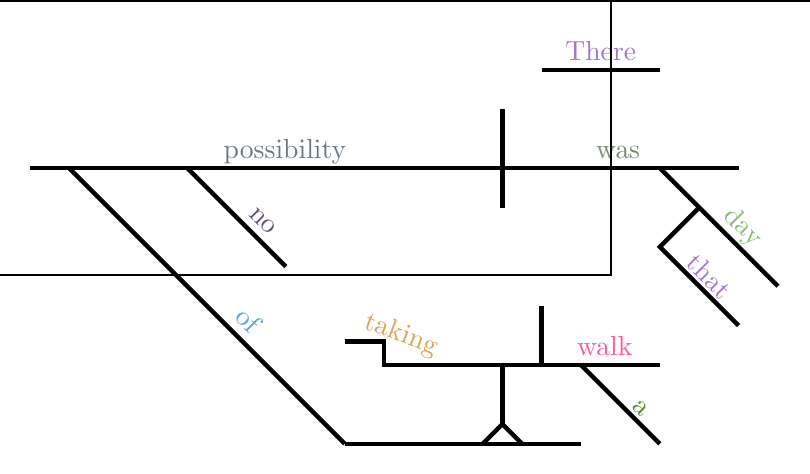
\begin{tikzpicture}
            \draw (3.5, 4.25) -- (5, 4.25)
                node[pos=0.5, text=pronoun]{\strut There};

            \draw (-3, 3) -- (6, 3)
                node[pos=0.36, text=subjectnoun]{\strut possibility}
                node[pos=0.83, text=copula]{\strut was};
            \draw (3, 3.75) -- (3, 2.5);
            \draw (-1, 3) -- (0.25, 1.75)
                node[sloped, pos=0.65, text=adjective]{\strut no};
            \draw (-2.5, 3) -- (1, -0.5)
                node[sloped, pos=0.6, text=preposition]{\strut of};

            \draw (5, 3) -- (6.5, 1.5)
                node[sloped, pos=0.6, text=adverb]{\strut day};
            \draw (5.5, 2.5) -- (5, 2) -- (6, 1)
                node[above=-0.06cm, sloped, pos=0.5, text=pronoun]{\strut that};

            \draw (1, -0.5) -- (4, -0.5);
            \draw (1, 0.8) -- (1.5, 0.8) -- (1.5, 0.5) -- (5, 0.5)
                node[pos=0.8, text=directobject]{\strut walk};
            \path (1.5, 0.8) -- (2.3, 0.5)
                node[above=-0.06cm, sloped, pos=0.2, text=verb]{\strut taking};
            \draw (4, 0.5) -- (5, -0.5)
                node[above=-0.06cm, sloped, pos=0.65, text=article]{\strut a};
            \draw (3.5, 0.5) -- (3.5, 1.25);
            \draw (3, 0.5) -- (3, -0.25);
            \draw (3, -0.25) -- (3.25, -0.5);
            \draw (3, -0.25) -- (2.75, -0.5);
        \end{tikzpicture}
    \end{sentencediagram}

    \begin{sentencediagram}{2.25}{2.5}{All this happened, more or less.}{Kurt Vonnegut}{Slaughterhouse Five}
        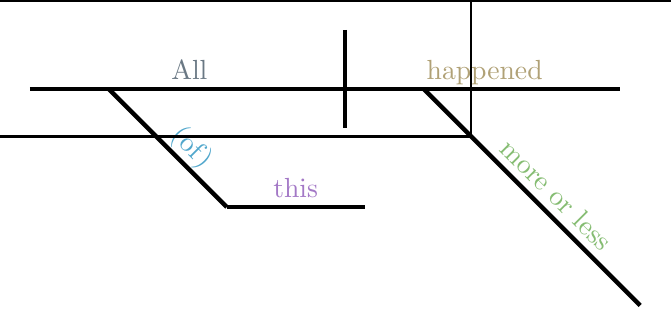
\begin{tikzpicture}
            \draw (-4.5, 2) -- (3, 2)
                node[pos=0.27, text=subjectnoun]{\strut All}
                node[pos=0.77, text=predicateverb]{\strut happened};
            \draw (-0.5, 2.75) -- (-0.5, 1.5);

            \draw (-3.5, 2) -- (-2, 0.5)
                node[sloped, pos=0.6, text=preposition]{\strut (of)};
            \draw (-2, 0.5) -- (-0.25, 0.5)
                node[pos=0.5, text=pronoun]{\strut this};
            \draw (0.5, 2) -- (3.25, -0.75)
                node[sloped, pos=0.55, text=adverb]{\strut more or less};
        \end{tikzpicture}
    \end{sentencediagram}

    \begin{sentencediagram}{2.25}{2.5}{Call me Ishmael.}{Herman Melville}{Moby Dick}
        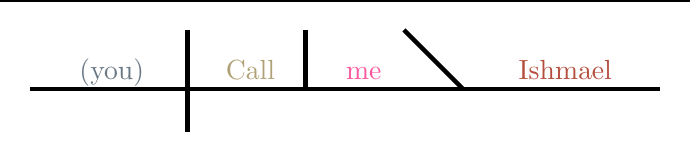
\begin{tikzpicture}
            \draw (-4, 0) -- (4, 0)
                node[pos=0.13, text=subjectnoun]{\strut (you)}
                node[pos=0.35, text=predicateverb]{\strut Call}
                node[pos=0.53, text=directobject]{\strut me}
                node[pos=0.85, text=noun]{\strut Ishmael};
            \draw (-2, 0.75) -- (-2, -0.55);
            \draw (-0.5, 0.75) -- (-0.5, 0);
            \draw (0.75, 0.75) -- (1.5, 0);
        \end{tikzpicture}
    \end{sentencediagram}

    \begin{sentencediagram}{2.25}{2.5}{It was a pleasure to burn.}{Ray Bradbury}{Fahrenheit 451}
        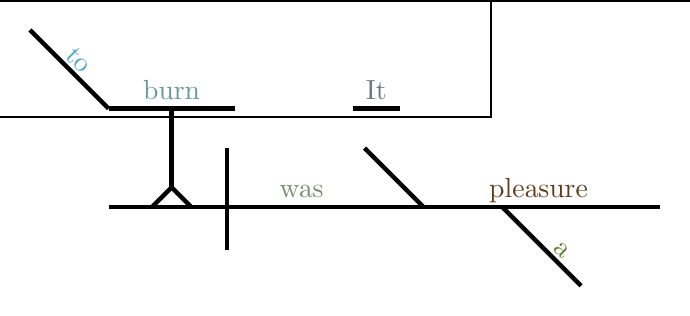
\begin{tikzpicture}
            \draw (0.1, 1.25) -- (0.7, 1.25)
                node[pos=0.5, text=subjectnoun]{\strut It};

            \draw (-4, 2.25) -- (-3, 1.25)
                node[above=-0.06cm, sloped, pos=0.5, text=preposition]{\strut to};
            \draw (-3, 1.25) -- (-1.4, 1.25)
                node[pos=0.5, text=infinitiveverb]{\strut burn};
            \draw (-2.2, 1.25) -- (-2.2, 0.25);
            \draw (-2.2, 0.25) -- (-1.95, 0);
            \draw (-2.2, 0.25) -- (-2.45, 0);

            \draw (-3, 0) -- (4, 0)
                node[pos=0.35, text=copula]{\strut was}
                node[pos=0.78, text=subjectcomplement]{\strut pleasure};
            \draw (-1.5, 0.75) -- (-1.5, -0.55);
            \draw (0.25, 0.75) -- (1, 0);
            \draw (2, 0) -- (3, -1)
                node[above=-0.06cm, sloped, pos=0.65, text=article]{\strut a};
        \end{tikzpicture}
    \end{sentencediagram}

    \begin{sentencediagram}{1.75}{2}{It was a bright cold day in April, and the clocks were striking thirteen.}{George Orwell}{1984}
        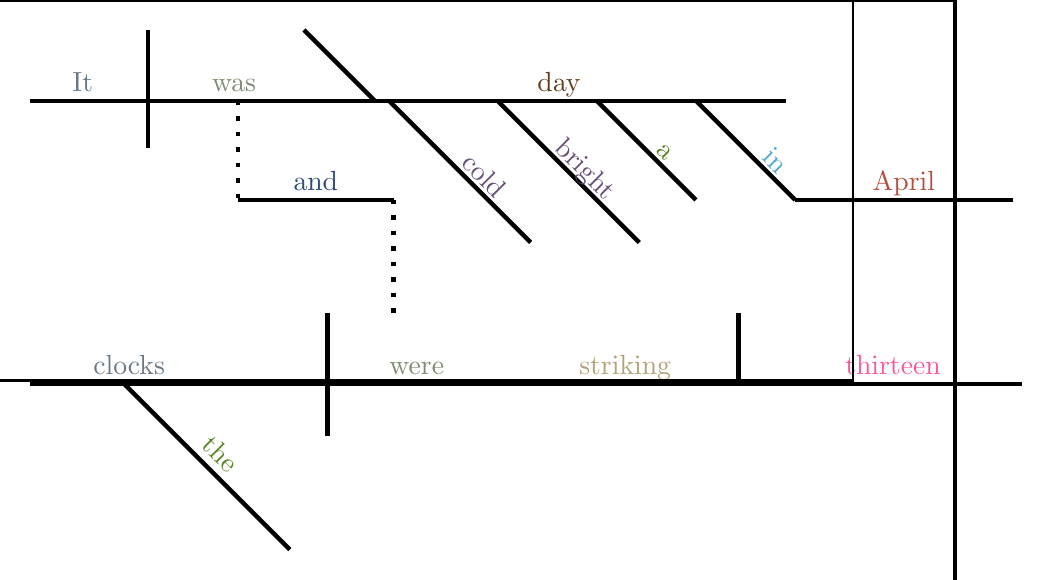
\begin{tikzpicture}[scale=1.2]
            \draw (-5, 1.75) -- (3, 1.75)
                node[pos=.07, text=subjectnoun]{\strut It}
                node[pos=.27, text=copula]{\strut was}
                node[pos=.7, text=subjectcomplement]{\strut day};
            \draw (-3.75, 2.5) -- (-3.75, 1.25);
            \draw (-2.1, 2.5) -- (-1.35, 1.75);
            \draw (-1.2, 1.75) -- (0.3, 0.25)
                node[above=-0.06cm, sloped, pos=0.6, text=adjective]{\strut cold};
            \draw (-0.05, 1.75) -- (1.45, 0.25)
                node[above=-0.06cm, sloped, pos=0.55, text=adjective]{\strut bright};
            \draw (1, 1.75) -- (2.05, 0.7)
                node[above=-0.06cm, sloped, pos=0.6, text=article]{\strut a};
            \draw (2.05, 1.75) -- (3.1, 0.7)
                node[above=-0.06cm, sloped, pos=0.7, text=preposition]{\strut in};

            \draw[loosely dotted] (-2.8, 1.75) -- (-2.8, 0.7);
            \draw (-2.8, 0.7) -- (-1.15, 0.7)
                node[pos=.5, text=conjunction]{\strut and};
            \draw (3.1, 0.7) -- (5.4, 0.7)
                node[pos=.5, text=noun]{\strut April};
            \draw[loosely dotted] (-1.15, 0.7) -- (-1.15, -0.5);

            \draw (-5, -1.25) -- (5.5, -1.25)
                node[pos=.1, text=subjectnoun]{\strut clocks}
                node[pos=.39, text=copula]{\strut were}
                node[pos=.6, text=predicateverb]{\strut striking}
                node[pos=.87, text=directobject]{\strut thirteen};
            \draw (-1.85, -0.5) -- (-1.85, -1.8);
            \draw (2.5, -1.25) -- (2.5, -0.5);
            \draw (-4, -1.25) -- (-2.25, -3.0)
                node[sloped, pos=.5, text=article]{\strut the};
        \end{tikzpicture}
    \end{sentencediagram}

    \begin{sentencediagram}{1.75}{2}{It is a truth universally acknowledged, that a single man\\in possession of a good fortune, must be in want of a wife.}{Jane Austen}{Pride and Prejudice}
        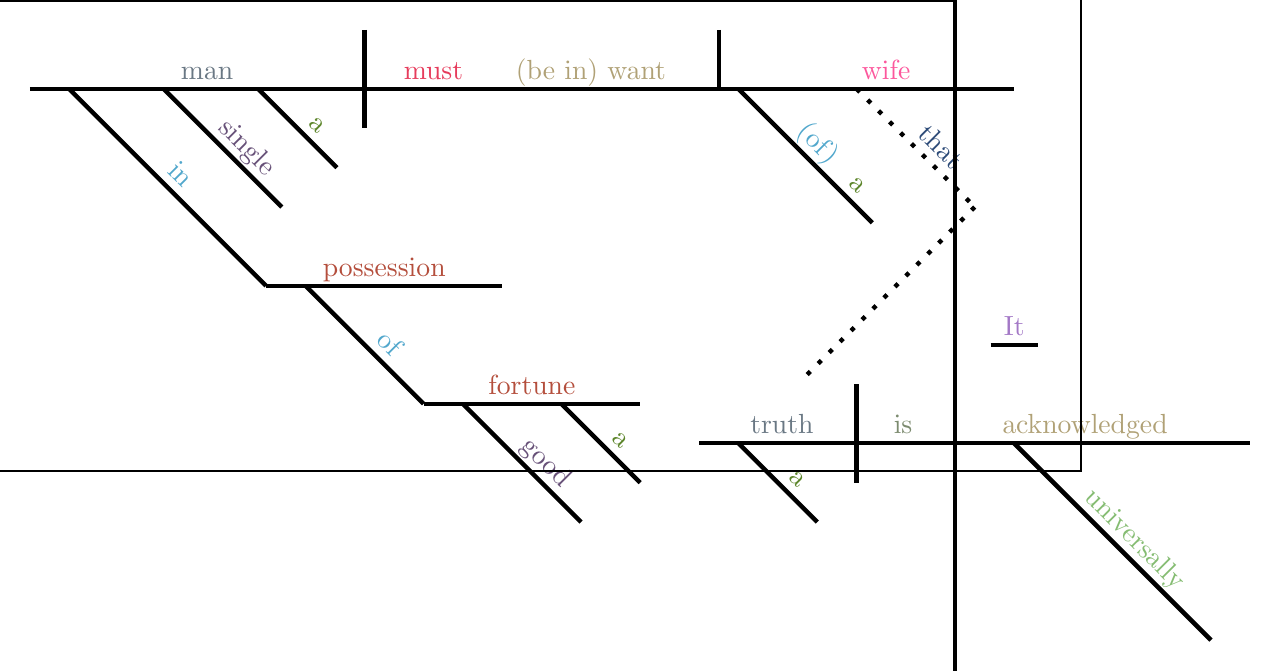
\begin{tikzpicture}
            \draw (5.7, -0.25) -- (6.3, -0.25)
                node[pos=0.5, text=pronoun]{\strut It};

            \draw (2, -1.5) -- (9, -1.5)
                node[pos=0.15, text=subjectnoun]{\strut truth}
                node[pos=0.37, text=copula]{\strut is}
                node[pos=0.7, text=predicateverb]{\strut acknowledged};
            \draw (2.5, -1.5) -- (3.5, -2.5)
                node[sloped, pos=0.6, text=article]{\strut a};
            \draw (4, -0.75) -- (4, -2);
            \draw (6, -1.5) -- (8.5, -4)
                node[sloped, pos=0.55, text=adverb]{\strut universally};

            \draw (-6.5, 3) -- (6, 3)
                node[pos=0.18, text=subjectnoun]{\strut man}
                node[pos=0.41, text=modalverb]{\strut must}
                node[pos=0.57, text=predicateverb]{\strut (be in) want}
                node[pos=0.87, text=directobject]{\strut wife};
            \draw (-2.25, 3.75) -- (-2.25, 2.5);
            \draw (2.25, 3.75) -- (2.25, 3);
            \draw (2.5, 3) -- (4.2, 1.3)
                node[sloped, pos=0.5, text=preposition]{\strut (of)}
                node[sloped, pos=0.8, text=article]{\strut a};
            \draw[loosely dotted] (4, 3) -- (5.5, 1.5)
                node[sloped, pos=0.6, text=conjunction]{\strut that};
            \draw[loosely dotted] (5.5, 1.5) -- (3.3, -0.7);

            \draw (-6, 3) -- (-3.5, 0.5)
                node[sloped, pos=0.5, text=preposition]{\strut in};
            \draw  (-4.8, 3) -- (-3.3, 1.5)
                node[sloped, pos=0.6, text=adjective]{\strut single};
            \draw (-3.6, 3) -- (-2.6, 2)
                node[sloped, pos=0.6, text=article]{\strut a};
            \draw (-3.5, 0.5) -- (-0.5, 0.5)
                node[pos=0.5, text=noun]{\strut possession};

            \draw (-3, 0.5) -- (-1.5, -1)
                node[sloped, pos=0.6, text=preposition]{\strut of};
            \draw (-1.5, -1) -- (1.25, -1)
                node[pos=0.5, text=noun]{\strut fortune};
            \draw (-1, -1) -- (0.5, -2.5)
                node[sloped, pos=0.6, text=adjective]{\strut good};
            \draw (0.25, -1) -- (1.25, -2)
                node[sloped, pos=0.6, text=article]{\strut a};
        \end{tikzpicture}
    \end{sentencediagram}

    \begin{sentencediagram}{1.75}{2}{Miss Brooke had that kind of beauty which seems to be thrown into relief by poor dress.}{George Eliot}{Middlemarch}
        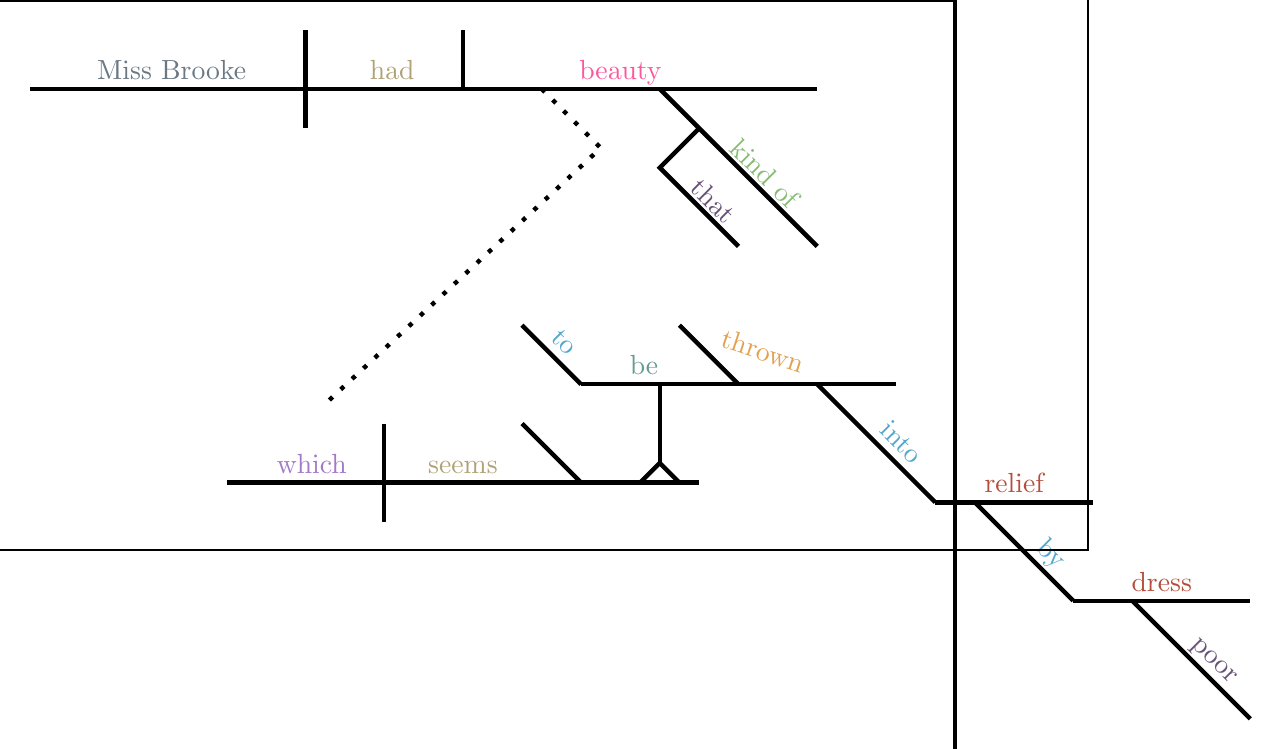
\begin{tikzpicture}
            \draw (-5, 3) -- (5, 3)
                node[pos=0.18, text=subjectnoun]{\strut Miss Brooke}
                node[pos=0.46, text=predicateverb]{\strut had}
                node[pos=0.75, text=directobject]{\strut beauty};
            \draw (-1.5, 3.75) -- (-1.5, 2.5);
            \draw (0.5, 3.75) -- (0.5, 3);
            \draw (3, 3) -- (5, 1)
                node[above=-0.06cm, sloped, pos=0.6, text=adverb]{\strut kind of};
            \draw (3.5, 2.5) -- (3, 2) -- (4, 1)
                node[above=-0.06cm, sloped, pos=0.55, text=adjective]{\strut that};
            \draw[loosely dotted] (1.5, 3) -- (2.25, 2.25) -- (-1.25, -1);

            \draw (-2.5, -2) -- (3.5, -2)
                node[pos=0.18, text=pronoun]{\strut which}
                node[pos=0.5, text=predicateverb]{\strut seems};
            \draw (-0.5, -1.25) -- (-0.5, -2.5);
            \draw (1.25, -1.25) -- (2, -2);

            \draw (1.25, 0) -- (2, -0.75)
                node[sloped, pos=0.5, text=preposition]{\strut to};
            \draw (2, -0.75) -- (6, -0.75)
                node[pos=0.2, text=infinitiveverb]{\strut be};
            \draw (3.25, 0) -- (4, -0.75);
            \path (3.5, -0.25) -- (5, -0.75)
                node[above=-0.06cm, sloped, pos=0.5, text=verb]{\strut thrown};
            \draw (3, -0.75) -- (3, -1.75);
            \draw (3, -1.75) -- (2.75, -2);
            \draw (3, -1.75) -- (3.25, -2);

            \draw (5, -0.75) -- (6.5, -2.25)
                node[sloped, pos=0.6, text=preposition]{\strut into};
            \draw (6.5, -2.25) -- (8.5, -2.25)
                node[pos=0.5, text=noun]{\strut relief};
            \draw (7, -2.25) -- (8.25, -3.5)
                node[sloped, pos=0.65, text=preposition]{\strut by};
            \draw (8.25, -3.5) -- (10.5, -3.5)
                node[pos=0.5, text=noun]{\strut dress};
            \draw (9, -3.5) -- (10.5, -5)
                node[sloped, pos=0.6, text=adjective]{\strut poor};
        \end{tikzpicture}
    \end{sentencediagram}

    \begin{sentencediagram}{1.75}{2}{It was a queer, sultry summer, the summer they electrocuted\\the Rosenbergs, and I didn't know what I was doing in New York}{Sylvia Plath}{The Bell Jar}
        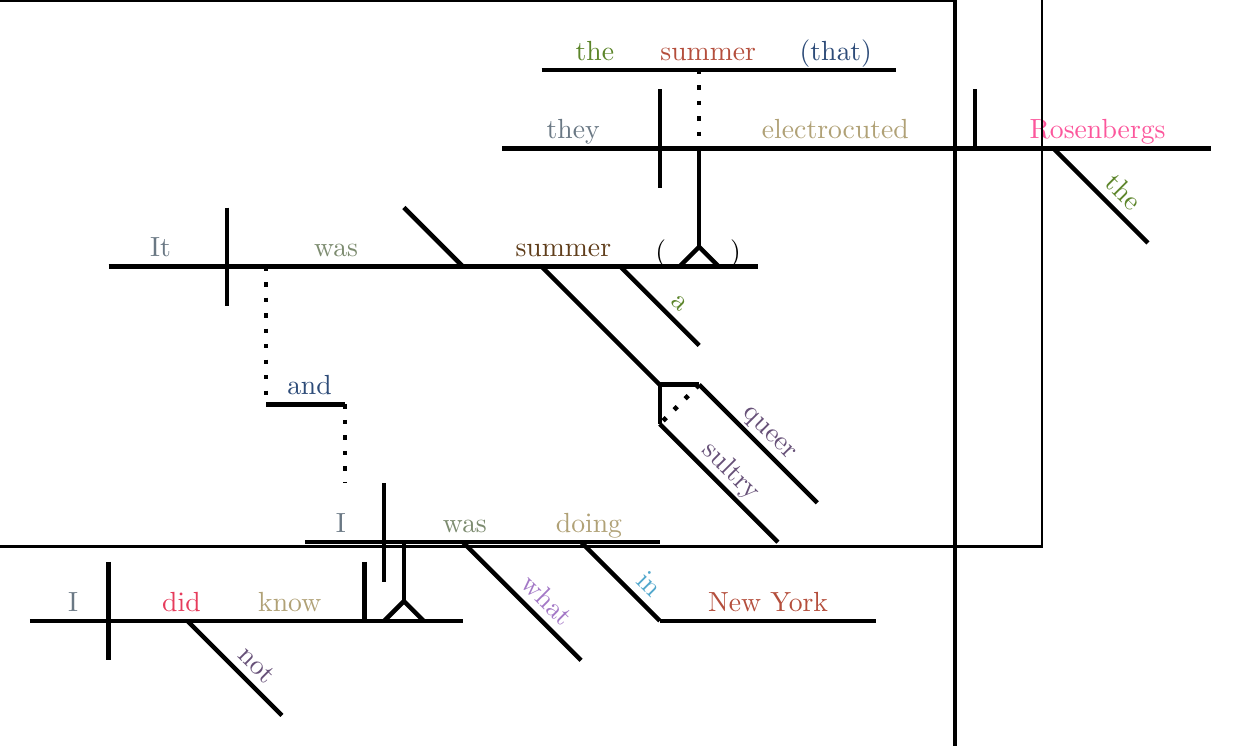
\begin{tikzpicture}
            \draw (-1.5, 3.5) -- (3, 3.5)
                node[pos=0.15, text=article]{\strut the}
                node[pos=0.47, text=noun]{\strut summer}
                node[pos=0.83, text=conjunction]{\strut (that)};
            \draw (-2, 2.5) -- (7, 2.5)
                node[pos=0.10, text=subjectnoun]{\strut they}
                node[pos=0.47, text=predicateverb]{\strut electrocuted}
                node[pos=0.84, text=directobject]{\strut Rosenbergs};
            \draw (0, 3.25) -- (0, 2);
            \draw[loosely dotted] (0.5, 3.5) -- (0.5, 2.5);
            \draw (4, 3.25) -- (4, 2.5);
            \draw (5, 2.5) -- (6.2, 1.3)
                node[sloped, pos=0.6, text=article]{\strut the};
            \draw (0.5, 2.5) -- (0.5, 1.25);
            \draw (0.5, 1.25) -- (0.25, 1);
            \draw (0.5, 1.25) -- (0.75, 1);

            \draw (-7, 1) -- (1.25, 1)
                node[pos=0.08, text=subjectnoun]{\strut It}
                node[pos=0.35, text=copula]{\strut was}
                node[pos=0.7, text=subjectcomplement]{\strut summer}
                node[pos=0.85]{(}
                node[pos=0.965]{)};
            \draw (-5.5, 1.75) -- (-5.5, 0.5);
            \draw (-3.25, 1.75) -- (-2.5, 1);
            \draw (-0.5, 1) -- (0.5, 0)
                node[sloped, pos=0.6, text=article]{\strut a};
            \draw (-1.5, 1) -- (0, -0.5);
            \draw (0, -0.5) -- (0.5, -0.5);
            \draw (0, -0.5) -- (0, -1);
            \draw[loosely dotted] (0.5, -0.5) -- (0, -1);
            \draw (0.5, -0.5) -- (2, -2)
                node[sloped, pos=0.5, text=adjective]{\strut queer};
            \draw (0, -1) -- (1.5, -2.5)
                node[sloped, pos=0.5, text=adjective]{\strut sultry};

            \draw[loosely dotted] (-5, 1) -- (-5, -0.75);
            \draw (-5, -0.75) -- (-4, -0.75)
                node[pos=0.55, text=conjunction]{\strut and};
            \draw[loosely dotted] (-4, -0.75) -- (-4, -1.75);

            \draw (-4.5, -2.5) -- (0, -2.5)
                node[pos=0.1, text=subjectnoun]{\strut I}
                node[pos=0.45, text=copula]{\strut was}
                node[pos=0.8, text=predicateverb]{\strut doing};
            \draw (-3.5, -1.75) -- (-3.5, -3);
            \draw (-2.5, -2.5) -- (-1, -4)
                node[sloped, pos=0.6, text=pronoun]{\strut what};
            \draw (-1, -2.5) -- (0, -3.5)
                node[sloped, pos=0.7, text=preposition]{\strut in};
            \draw (0, -3.5) -- (2.75, -3.5)
                node[pos=0.5, text=noun]{\strut New York};
            \draw (-3.25, -2.5) -- (-3.25, -3.25);
            \draw (-3.25, -3.25) -- (-3.5, -3.5);
            \draw (-3.25, -3.25) -- (-3, -3.5);

            \draw (-8, -3.5) -- (-2.5, -3.5)
                node[pos=0.1, text=subjectnoun]{\strut I}
                node[pos=0.35, text=modalverb]{\strut did}
                node[pos=0.6, text=predicateverb]{\strut know};
            \draw (-7, -2.75) -- (-7, -4);
            \draw (-3.75, -2.75) -- (-3.75, -3.5);
            \draw (-6, -3.5) -- (-4.8, -4.7)
                node[sloped, pos=0.6, text=adjective]{\strut not};
        \end{tikzpicture}
    \end{sentencediagram}

    \begin{sentencediagram}{0.25}{0.5}{The studio was filled with the rich odour of roses, and when the light summer wind stirred amidst the trees of the garden,\\there came through the open door the heavy scent of the lilac, or the more delicate perfume of the pink-flowering thorn.}{Oscar Wilde}{The Picture of Dorian Gray}
        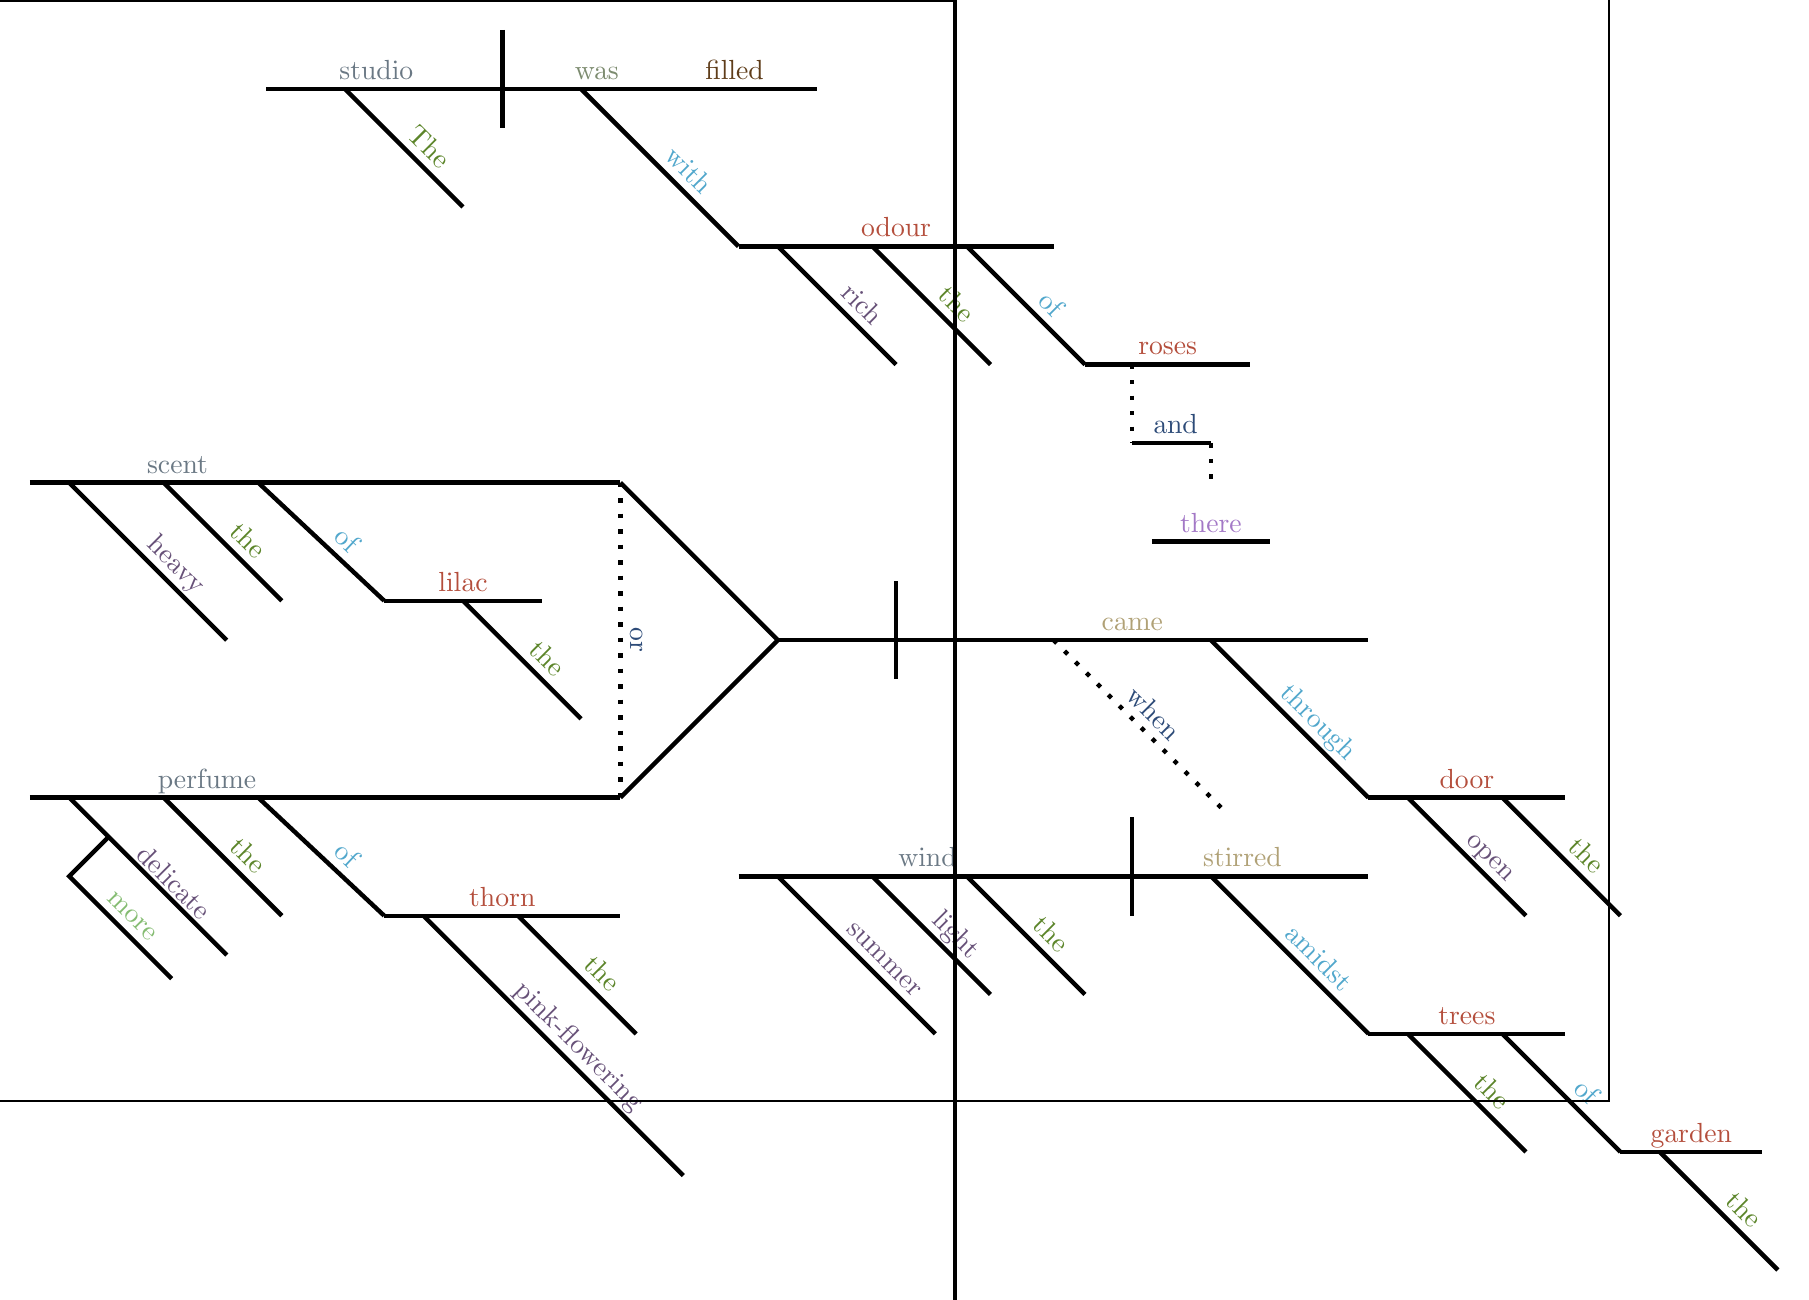
\begin{tikzpicture}
            \draw (-12, 8) -- (-5, 8)
                node[pos=0.2, text=subjectnoun]{\strut studio}
                node[pos=0.6, text=copula]{\strut was}
                node[pos=0.85, text=subjectcomplement]{\strut filled};
            \draw (-9, 8.75) -- (-9, 7.5);
            \draw (-11, 8) -- (-9.5, 6.5)
                node[sloped, pos=0.6, text=article]{\strut The};
            \draw (-8, 8) -- (-6, 6)
                node[sloped, pos=0.6, text=preposition]{\strut with};
            \draw (-6, 6) -- (-2, 6)
                node[pos=0.5, text=noun]{\strut odour};
            \draw (-5.5, 6) -- (-4, 4.5)
                node[sloped, pos=0.6, text=adjective]{\strut rich};
            \draw (-4.3, 6) -- (-2.8, 4.5)
                node[sloped, pos=0.6, text=article]{\strut the};
            \draw (-3.1, 6) -- (-1.6, 4.5)
                node[sloped, pos=0.6, text=preposition]{\strut of};
            \draw (-1.6, 4.5) -- (0.5, 4.5)
                node[pos=0.5, text=noun]{\strut roses};

            \draw [loosely dotted] (-1, 4.5) -- (-1, 3.5);
            \draw (-1, 3.5) -- (0, 3.5)
                node[pos=0.55, text=conjunction]{\strut and};
            \draw [loosely dotted] (0, 3.5) -- (0, 3);

            \draw (-15, 3) -- (-7.5, 3)
                node[pos=0.25, text=subjectnoun]{\strut scent};
            \draw (-14.5, 3) -- (-12.5, 1)
                node[sloped, pos=0.6, text=adjective]{\strut heavy};
            \draw (-13.3, 3) -- (-11.8, 1.5)
                node[sloped, pos=0.6, text=article]{\strut the};
            \draw (-12.1, 3) -- (-10.5, 1.5)
                node[sloped, pos=0.6, text=preposition]{\strut of};
            \draw (-10.5, 1.5) -- (-8.5, 1.5)
                node[pos=0.5, text=noun]{\strut lilac};
            \draw (-9.5, 1.5) -- (-8, 0)
                node[sloped, pos=0.6, text=article]{\strut the};

            \draw (-7.5, 3) -- (-5.5, 1) -- (-7.5, -1);
            \draw [loosely dotted] (-7.5, 3) -- (-7.5, -1)
                node[sloped, pos=0.5, text=conjunction]{\strut or};

            \draw (-15, -1) -- (-7.5, -1)
                node[pos=0.3, text=subjectnoun]{\strut perfume};
            \draw (-14.5, -1) -- (-12.5, -3)
                node[above=-0.06cm, sloped, pos=0.6, text=adjective]{\strut delicate};
            \draw (-14, -1.5) -- (-14.5, -2) -- (-13.2, -3.3)
                node[sloped, pos=0.5, text=adverb]{\strut more};
            \draw (-13.3, -1) -- (-11.8, -2.5)
                node[sloped, pos=0.6, text=article]{\strut the};
            \draw (-12.1, -1) -- (-10.5, -2.5)
                node[sloped, pos=0.6, text=preposition]{\strut of};
            \draw (-10.5, -2.5) -- (-7.5, -2.5)
                node[pos=0.5, text=noun]{\strut thorn};
            \draw (-10, -2.5) -- (-6.7, -5.8)
                node[sloped, pos=0.55, text=adjective]{\strut pink-flowering};
            \draw (-8.8, -2.5) -- (-7.3, -4)
                node[sloped, pos=0.6, text=article]{\strut the};
            
            \draw (-0.75, 2.25) -- (0.75, 2.25)
                node[pos=0.5, text=pronoun]{\strut there};
            \draw (-5.5, 1) -- (2, 1)
                node[pos=0.6, text=predicateverb]{\strut came};
            \draw (-4, 1.75) -- (-4, 0.5);
            \draw [loosely dotted] (-2, 1) -- (0.2, -1.2)
                node[sloped, pos=0.5, text=conjunction]{\strut when};
            \draw (0, 1) -- (2, -1)
                node[sloped, pos=0.6, text=preposition]{\strut through};
            \draw (2, -1) -- (4.5, -1)
                node[pos=0.5, text=noun]{\strut door};
            \draw (2.5, -1) -- (4, -2.5)
                node[sloped, pos=0.6, text=adjective]{\strut open};
            \draw (3.7, -1) -- (5.2, -2.5)
                node[sloped, pos=0.6, text=article]{\strut the};

            \draw (-6, -2) -- (2, -2)
                node[pos=0.3, text=subjectnoun]{\strut wind}
                node[pos=0.8, text=predicateverb]{\strut stirred};
            \draw (-5.5, -2) -- (-3.5, -4)
                node[sloped, pos=0.6, text=adjective]{\strut summer};
            \draw (-4.3, -2) -- (-2.8, -3.5)
                node[sloped, pos=0.6, text=adjective]{\strut light};
            \draw (-3.1, -2) -- (-1.6, -3.5)
                node[sloped, pos=0.6, text=article]{\strut the};
            \draw (-1, -1.25) -- (-1, -2.5);
            \draw (0, -2) -- (2, -4)
                node[sloped, pos=0.6, text=preposition]{\strut amidst};
            \draw (2, -4) -- (4.5, -4)
                node[pos=0.5, text=noun]{\strut trees};
            \draw (2.5, -4) -- (4, -5.5)
                node[sloped, pos=0.6, text=article]{\strut the};
            \draw (3.7, -4) -- (5.2, -5.5)
                node[sloped, pos=0.6, text=preposition]{\strut of};
            \draw (5.2, -5.5) -- (7, -5.5)
                node[pos=0.5, text=noun]{\strut garden};
            \draw (5.7, -5.5) -- (7.2, -7)
                node[sloped, pos=0.6, text=article]{\strut the};
        \end{tikzpicture}
    \end{sentencediagram}
\end{document}
